\newcommand{\rev}{01 - 23-Jul-2021}
% REV01 Fri 23 Jul 2021 16:51:45 WIB
% START Fri 26 Mar 2021 12:10:02 WIB

\documentclass[12pt]{book}
\usepackage[a4paper, margin=50pt]{geometry}
\usepackage[dvipsnames,table,xcdraw]{xcolor}
\usepackage{colortbl}
\usepackage[hidelinks]{hyperref}
\usepackage[pdftex]{graphicx}
\definecolor{links}{HTML}{0011FF}
\hypersetup{colorlinks,linkcolor=,urlcolor=links}

% Should be loaded after the hyperref and bookmark packages
\usepackage{chngcntr}
\counterwithin*{chapter}{part}
% \counterwithout{chapter}{part}

\newcommand{\pengarangs}{%
    Dickens McCartney\\
}
\newcommand{\judul}{%
Jenny Wren\\[13pt]
Our Mutual Friend
}

\begin{document}

\begin{titlepage}
    \begin{center}    

    \vspace*{15mm}
    \textbf{\Large \judul}

    \vspace*{30mm}       
    \textbf{by}

    \vspace*{15mm}    
    \textbf{\Large \pengarangs}

    \vspace*{4.0cm}

    \begin{center}
        
\includegraphics[width=40mm]{ucls-coat}
    \end{center}

    \textbf{
       Universe Centra Le Sahara (UCLS)\\[10pt]
       Omar Bakry School of Management\\[10pt]
       Jabal Acacus Campus, Ghat. \\[10pt]
       \url{https://jennywren.vlsm.org/} \\[10pt]
       Rev. \rev%
    }

    %\vspace*{5mm}    
    %\textbf{\LARGE \textcolor{red}{***** Work In Progress *****}}

    \end{center}

\end{titlepage}

\pagenumbering{roman}

\tableofcontents

\newpage

\chapter*{Jenny Wren}
\addcontentsline{toc}{chapter}{Jenny Wren}

\begin{verbatim}
Like so many girls
Jenny Wren could sing
But a broken heart
Took her soul away

--- Dickens McCartney
\end{verbatim}

\noindent
Jenny Wren lyrics \copyright MPL Communications Ltd. See also \url{https://jennywren.vlsm.org/}.
\\[1pt]

\noindent
Jenny Wren --- whose real name is Fanny Cleaver,
is ''the dolls' dressmaker'' with whom Lizzie lives after her father dies.
She is crippled with a bad back, although not ugly.
She is very motherly towards her drunken father, whom she calls her ''bad child''.
Jenny later cares for Eugene while he recovers from Headstone's attack on his life.
She may have a romance with Sloppy at the end of the book,
which the reader may surmise will end in marriage.
Although her mannerisms give her a certain ''strangeness'', Jenny is very perceptive,
identifying Eugene Wrayburn's intentions towards Lizzie in his small actions.
Her role is a creator and a caretaker, 
and her ''pleasant fancies'' of ''flowers, bird song, numbers of blessed, 
white-clad children'' reflect the mind's ability to rise above adverse 
circumstances --- \url{https://en.wikipedia.org/wiki/Jenny_Wren}
\\[1pt]

\noindent
Jenny Wren aka Fanny Cleaver --- Sharp and sassy maker of doll's clothes, 
pincushions, and pen-wipers. 
Crippled (my back’s bad, and my legs are queer),
she lives with her drunken father whom she refers to as her bad child.
Lizzie Hexam, after the death of her father,
takes lodging with Jenny who helps Lizzie escape London when pursued by Bradley Headstone and Eugene Wrayburn.
It was difficult to guess the age of this strange creature,
for her poor figure furnished no clue to it,
and her face was at once so young and so old. Twelve,
or at the most thirteen, might be near the mark --- 
\url{https://www.charlesdickenspage.com/dickens-characters-t-z.html}
\\[1pt]

\noindent
=== Rev. \rev ===

\newpage

\pagenumbering{arabic}

\part{Book the First:\\THE CUP AND THE LIP}
% REV01 Thu 05 Aug 2021 14:26:40 WIB
% START Tue 03 Aug 2021 13:44:15 WIB

\chapter{Remodeling Grounded Theory}

\section*{Abstract}
\addcontentsline{toc}{section}{Abstract}

This paper outlines my concerns with Qualitative Data Analysis (QDA)
numerous remodelings of Grounded Theory (GT) and the subsequent eroding
impact. I cite several examples of the erosion and summarize essential
elements of classic GT methodology. It is hoped that the article will clarify my
concerns with the continuing enthusiasm but misunderstood embrace of GT by
QDA methodologists and serve as a preliminary guide to novice researchers
who wish to explore the fundamental principles of GT.

\begin{quote}
''Today’s general textbooks perpetuate the established marketing
management epic from the 1960s with the new just added as extras. It
is further my contention that marketing education has taken an
unfortunate direction and has crossed the fine line between education
and brainwashing. The countdown of a painful—but revitalizing—
process of deprogramming has to be initiated.

What do we need in such a situation? A shrink? No, it is less
sophisticated than that. All we need is systematic application of
common sense, both in academe and in corporations.We need to use
our observational capacity in an inductive mode and allow it to receive
the true story of life, search for patterns and build theory.Yes, theory.
General marketing theory that helps us put events and activities into a
context. This is all within the spirit of grounded theory, wide spread in
sociology but little understood by marketers. My interpretation of a
recent book on the subject by 
\citep{book.glaser01}
is as follows: ‘take the
elevator from the ground floor of raw substantive data and description to
the penthouse of conceptualization and general theory. And do this
without paying homage to the legacy of extant theory.’ In doing this,
complexity, fuzziness and ambiguity are received with cheers by the
researchers and not shunned as unorderly and threatening as they are
by quantitative researchers. Good theory is useful for scholars and
practicing managers alike \citep[p. 132]{article.gummensson02}.''
\end{quote}

\nocite{article.cynthia10}.
\bibliographystyle{apalikerd}
\bibliography{bib}


\part{Book The Second:\\BIRDS OF A FEATHER}
% REV01 Tue 03 Aug 2021 13:44:15 WIB
% START Tue 03 Aug 2021 13:44:15 WIB

\chapter{StarBucks Ipsum}

StarBucks ipsum dolor J.CO Do Not!
McD ipsum dolor Wendy’s Burger King.
KFC urna libero, in purus hana masa, sore wa tempura hokben.

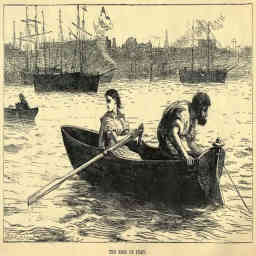
\includegraphics[scale=2.3]{01-01-01}

StarBucks ipsum dolor J.CO Do Not!
McD ipsum dolor Wendy’s Burger King.
KFC urna libero, in purus hana masa, sore wa tempura hokben.

\part{Book The Third:\\A LONG LANE}
% REV01 Tue 03 Aug 2021 13:44:15 WIB
% START Tue 03 Aug 2021 13:44:15 WIB

\chapter{StarBucks Ipsum}

StarBucks ipsum dolor J.CO Do Not!
McD ipsum dolor Wendy’s Burger King.
KFC urna libero, in purus hana masa, sore wa tempura hokben.

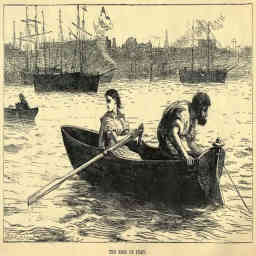
\includegraphics[scale=2.3]{01-01-01}

StarBucks ipsum dolor J.CO Do Not!
McD ipsum dolor Wendy’s Burger King.
KFC urna libero, in purus hana masa, sore wa tempura hokben.

\part{Book The Fourth:\\A TURNING}
% REV02 Fri 23 Jul 2021 17:19:30 WIB
% REV01 Sun 27 Jun 2021 07:29:17 WIB
% START Tue 04 May 2021 13:55:16 WIB

\chapter{SETTING TRAPS}

Plashwater Weir Mill Lock looked tranquil and pretty on an evening in
the summer time. A soft air stirred the leaves of the fresh green trees,
and passed like a smooth shadow over the river, and like a smoother
shadow over the yielding grass. The voice of the falling water, like
the voices of the sea and the wind, were as an outer memory to a
contemplative listener; but not particularly so to Mr Riderhood, who sat
on one of the blunt wooden levers of his lock-gates, dozing. Wine must
be got into a butt by some agency before it can be drawn out; and the
wine of sentiment never having been got into Mr Riderhood by any agency,
nothing in nature tapped him.



\part{Take Note!}
\thispagestyle{plain}

\chapter*{Disclaimer}

\section*{Terms and Conditions}

You should follow the terms and conditions of these following links:
\begin{itemize}
\item \url{https://www.gutenberg.org/files/883/883-h/883-h.htm}
\item \url{https://www.charlesdickenspage.com/}
\item \url{https://www.paulmccartney.com/albums/songs/jenny-wren}
\begin{itemize}
\item Jenny Wren lyrics \copyright MPL Communications Ltd.
\end{itemize}
\end{itemize}

\noindent
This ebook is just humorous intention of fighting the 2020-2021 lockdown boredom.
I believe this is \textbf{FAIR USE}, but I am not a lawyer.
My apology to Sir Paul McCartney, Charles Dickens, and Project Gutenberg, duh!

\section*{Project Gutenberg}

Produced by Donald Lainson and David Widger.

Creating the works from public domain print editions means that no
one owns a United States copyright in these works, so the Foundation
(and you!) can copy and distribute it in the United States without
permission and without paying copyright royalties.  Special rules,
set forth in the General Terms of Use part of this license, apply to
copying and distributing Project Gutenberg$^{tm}$ electronic works to
protect the PROJECT GUTENBERG$^{tm}$ concept and trademark.  Project
Gutenberg is a registered trademark, and may not be used if you
charge for the eBooks, unless you receive specific permission.  If you
do not charge anything for copies of this eBook, complying with the
rules is very easy.  You may use this eBook for nearly any purpose
such as creation of derivative works, reports, performances and
research.  They may be modified and printed and given away--you may do
practically ANYTHING with public domain eBooks.  Redistribution is
subject to the trademark license, especially commercial redistribution.


\subsection*{THE FULL PROJECT GUTENBERG LICENSE PLEASE READ THIS BEFORE YOU DISTRIBUTE OR USE THIS WORK}

To protect the Project Gutenberg$^{tm}$ mission of promoting the free
distribution of electronic works, by using or distributing this work
(or any other work associated in any way with the phrase “Project
Gutenberg”), you agree to comply with all the terms of the Full Project
Gutenberg$^{tm}$ License (available with this file or online at
\url{http://gutenberg.org/license}).

Yada yada yada...



% %%%%%%%%%%%%%%%%
\end{document}%%%%
% End of document.
% %%%%%%%%%%%%%%%%

